\begin{frame}[shrink=20,fragile]
  \frametitle{The FEniCS challenge!}
  \begin{columns}[c]
    \begin{column}{0.5\textwidth}
    Solve
          \vspace{-1em}
          \begin{align*}
            -\nabla \cdot (k_1(x,y) \nabla u) + u  &= f \quad \text{in
          } \Omega_1 \\
            -\nabla \cdot (k_2(x,y) \nabla u) &= f \quad \text{in }
              \Omega_2 
          \end{align*}
          \vspace{-2.0em}
          \begin{align*}
                    u &= g_D \quad \text{on } \partial \Omega_D \\
            -\dfrac{\partial u}{\partial \bfn} &= g_{N,1} \quad \text{on }
            \partial \Omega_{N,1} \\
            -\dfrac{\partial u}{\partial \bfn} &= u - g_{N,2} \quad \text{on }
            \partial \Omega_{N,2}
          \end{align*}
    by first finding the weak formulation and then solving the system
    numerically using \text{FEniCS}
    \end{column}
    \begin{column}{0.5\textwidth}
      \begin{center}
        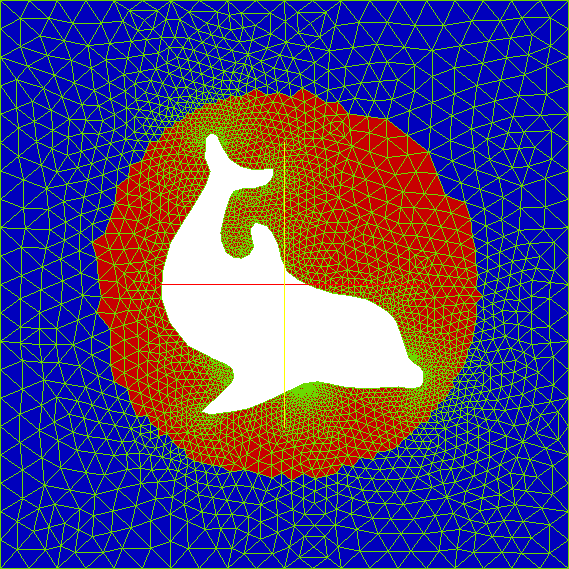
\includegraphics[width=1.0\textwidth]{png/poisson_5_subdomains.png}
      \end{center}
    \end{column}
  \end{columns}
  \begin{block}{Tools}
    Define facet markers
    \vspace{-1em}
    \begin{python}
boundary_markers = FacetFunction("size_t",mesh)
...
    \end{python}
    A redefinition of ``ds'' is necessary as well (why?). How will that probably look
    like? 
\end{block}
\end{frame}
